\documentclass[11pt, fleqn]{article}

\usepackage[letterpaper, margin=0.7in]{geometry}
\usepackage{graphicx}
\usepackage{subcaption}
\usepackage{cleveref}
\usepackage{listings}
\usepackage{multicol}
\usepackage{tikz}
\usepackage{bm}
\usepackage{minted}
\usetikzlibrary{arrows}
\usepackage{wrapfig}
\usepackage{amsmath}
\usepackage{amssymb}
\usepackage[section]{placeins}
\usepackage{pgfplots,wrapfig}  
\pgfplotsset{compat=newest} 
\pgfplotsset{plot coordinates/math parser=false} 
\newlength\figureheight 
\newlength\figurewidth 
\setlength{\parindent}{0pt}
\newcommand\tab[1][1cm]{\hspace*{#1}}
\usepackage{algorithm}
\usepackage[noend]{algpseudocode}

\let\oldReturn\Return
\renewcommand{\Return}{\State\oldReturn}

\raggedbottom

\begin{document}

\begin{center}

\Large{COMP6212 Assignment 4 : Shakib-Bin Hamid 25250094 sh3g12}

\end{center}

\section{Kalman Filter}

Lets suppose a data generative process is a linear combination of its past values, i.e. the current process process parameters are a linear combination of previous process parameters. In this respect we can calculate the process parameters by minimising the least squared error between the prediction and the true values, $\bm{\omega} = (\bm{Y}^t\bm{Y})^{-1}\bm{Y}^t\bm{f}$, where $\bm{Y}$ is the input data and $\bm{f}$ is the target. But this method requires calculating a new $\bm{Y}^{-1}$ (a $O(n^3)$ operation) when we receive any new data. If the process is generating a time series data (getting data one at a time), then online updating the parameters can be incredibly costly.\\

However, it can be shown that we can calcuate new parameters without calculating a new inverse, $\bm{\omega}_n = \bm{\omega}_{n-1} + L \times (f_n - \bm{\omega}_{n-1}^t\bm{y_n})$. It means that we can calculate new parameters by updating the old parameters with the scaled prediction error on new data using the old parameters. Of course we need to assume some initial values for our parameters. But, we still do not account for any noise in our process.\\

In a Kalman Filter, we may assume a process $\bm{\omega}_n = \bm{A}\bm{\omega}_{n-1} + \bm{\epsilon}(n)$, where the process noise $\bm{\epsilon} \sim \mathcal{N}(0, \bm{Q})$. Here we can assume that our parameters are a linear transformation of previous parameters corrupted by Gaussian noise. Similarly, we can assume that our observation $f_n = \bm{\omega}_n\bm{y}_n + \xi(n)$, where observation noise $\xi \sim \mathcal{N}(0, R)$.\\

\cite{mahler} claims that we can predict the monthly S\&P 500 index using a Kalman filter. In order to verify his claim, I have implemented Algorithm \ref{alg:kalman} -

\begin{algorithm}[H]
\caption{S\&P 500 Index Prediction using a Kalman Filter}
\label{alg:kalman}
\begin{algorithmic}[1]

\Procedure{Kalman}{$\bm{s}, o, \alpha$} \Comment{$\bm{s}$ = index, $o$ = order, $\alpha$ = a constant}

\State

\State $N$ = $size(\bm{s}, 1)$; \Comment{Number of months}
\State $\bm{Y}$ = $zeros(N - o + 1, o)$; \Comment{Input data in $o$ order windows}
\State $\bm{W}$ = $zeros(N, o)$; \Comment{Weights at every point}
\State $\bm{e}$ = $zeros(N - o + 1, 1)$; \Comment{Prediction error at every point}

\State

\State $m$ = $ar(s, o)$; \Comment{Matlab's autoregression function}
\State $R$ = $m.NoiseVariance$; \Comment{Observation noise variance}
\State $\bm{w}$ = $(m.a(2:o+1) \times -1)^t$; \Comment{Current weight set to initial value}

\State

\State $\bm{A}$ = $\bm{I}_o$ \Comment{$\bm{I}_o$ is the $o$ order Identity}
\State $\bm{Q}$ = $\alpha\bm{I}_o$ \Comment{Process noise covariance}
\State $\bm{P}$ = $\bm{I}_o$ \Comment{Uncertainity or covariance of parameters}

\State

\For {$n \gets o + 1,N$}

	\State $\bm{y}_n$ = $\bm{Y}(n, :)$ = $\bm{s}(n - o:n - 1)$ \Comment{Input is last $o$ months' index}

	\State

	\State $\bm{P}$ = $\bm{A}\bm{P}\bm{A}^t$ + $\bm{Q}$ \Comment{Uncertainity on parameters increases}

	\State
	
	\State $\bm{e}(n)$ = $\bm{s}(n)$ - $\bm{w}^t\bm{y}_n$ \Comment{Prediction Error}
	\State $\bm{K}$ = $\bm{P}\bm{y}_n/(R + \bm{y}_n^t\bm{P}\bm{y}_n)$ \Comment{Kalman Gain}

	\State

	\State $\bm{w} = \bm{W}(n, :)$ = $\bm{w} + \bm{K}\bm{e}(n)$ \Comment{Correction}
	\State $\bm{P}$ = $(\bm{I}_o - \bm{K}\bm{y}_n^t)\bm{P}$ 

\EndFor

\EndProcedure
\end{algorithmic}
\end{algorithm}

\begin{wrapfigure}{!h}{0.5\textwidth}
  	\centering
  	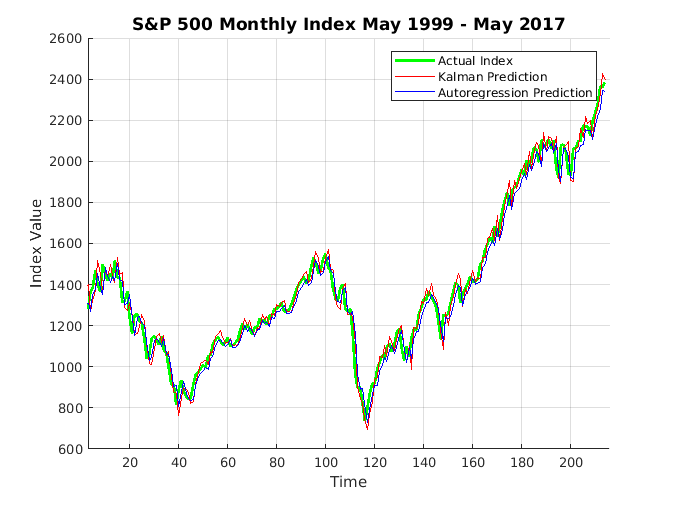
\includegraphics[width=0.5\textwidth]{kalman-autoreg-pred.png}
	\caption{Kalman \& Autoregression Prediction}
	\label{fig:kalman-autoreg-pred}
	\vspace{-1cm}
\end{wrapfigure}

The input at each point in time is past $o$ index values. Observation noise $R$ is taken as the residual variance from an autoregression model using \texttt{ar} function of Matlab's System Identification Toolbox. Process noise covariance needed to be tuned via $\alpha$. Figure \ref{fig:error-vs-alpha-order-3} (where I have plotted the cumulative sum of prediction error as a function of $\alpha$ for a 3rd order filter), indicates that $10^{-3}$ is a reasonable value for $\alpha$. Unless otherwise specified, it can be assumed that a 3rd order filter and autoregression was in use. The parameters were initialised in Line 10 and covariance in Line 14.\\

\begin{figure}[!h]
    \centering
    \begin{subfigure}[b]{0.45\textwidth}
        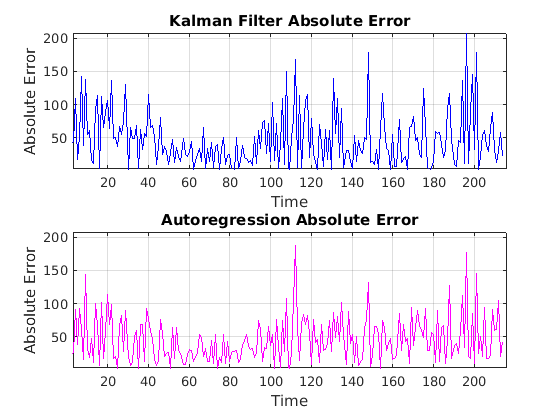
\includegraphics[width=\textwidth]{kalman-autoreg-error.png}
		\caption{Index Prediction Absolute Error}
		\label{fig:kalman-autoreg-error}
    \end{subfigure}
    ~ 
    \begin{subfigure}[b]{0.42\textwidth}
        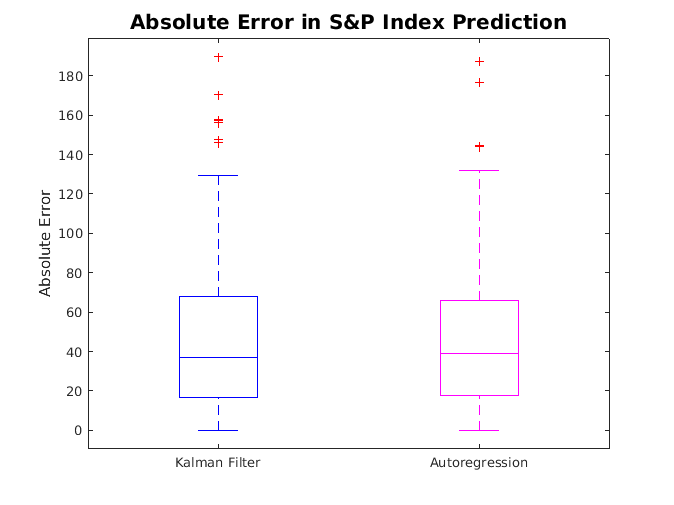
\includegraphics[width=\textwidth]{kalman-autoreg-error-boxplot.png}
		\caption{Index Prediction Error Comparison}
		\label{fig:kalman-autoreg-error-boxplot}
    \end{subfigure}
    \caption{Prediction Error}
	\label{fig:prediction-error}
\end{figure}

I began by generating an artificial time series using white Gaussian noise (Matlab's \texttt{wgn} function) and $(0.5, 0.6, 0.1)$ weights. The kalman filter quickly stabilises on this data at the expected weights (Figure \ref{fig:kalman-parameter-converge-artificial}). After confirming the correctness of the kalman filter, I applied it to real data.\\

Figure \ref{fig:kalman-autoreg-pred} is showing the monthly index values, as well as prediction made from an autoregression and the implemented Kalman filter. Clearly both are very close to the true values of the index. We can also see from Figure \ref{fig:kalman-autoreg-error} that both methods produce very similar error patterns. Figure \ref{fig:kalman-autoreg-error-boxplot} shows that the errors have very similar spread.\\


\begin{figure}[!h]
    \centering
	\begin{subfigure}[b]{0.28\textwidth}
        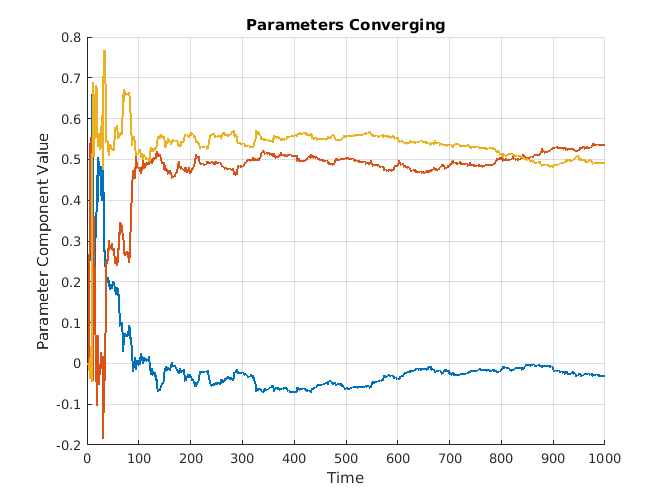
\includegraphics[width=\textwidth]{kalman-parameter-converge-artificial.png}
	\caption{Artifical}
	\label{fig:kalman-parameter-converge-artificial}
    \end{subfigure}
    ~ 
    \begin{subfigure}[b]{0.28\textwidth}
        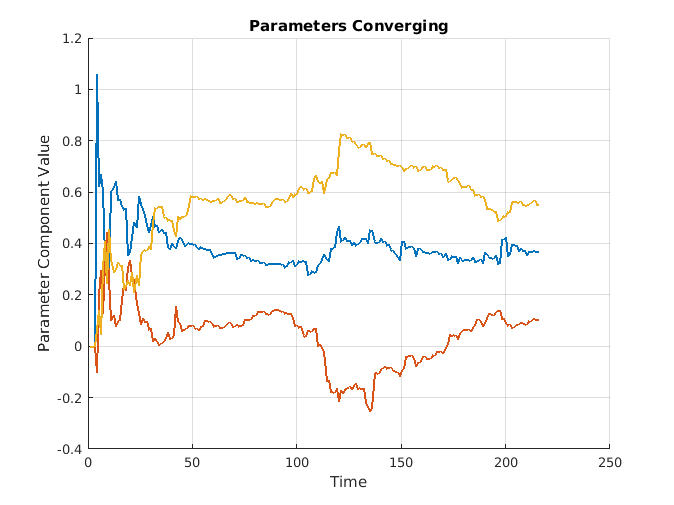
\includegraphics[width=\textwidth]{kalman-parameter-converge.png}
		\caption{$R \approx 53$}
		\label{fig:kalman-parameter-converge}
    \end{subfigure}
	~ 
    \begin{subfigure}[b]{0.3\textwidth}
        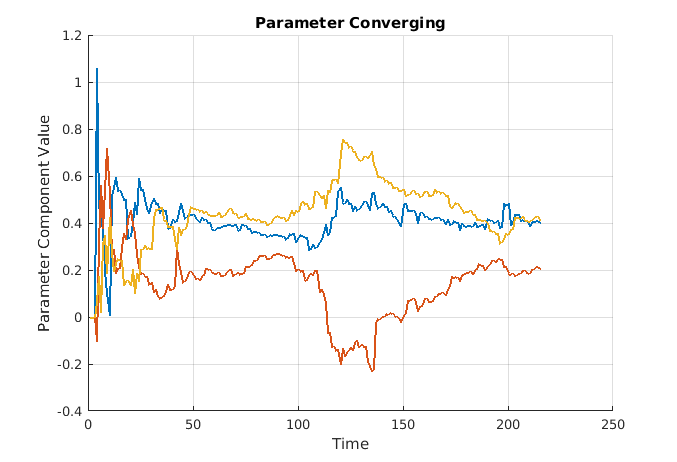
\includegraphics[width=\textwidth]{kalman-parameter-converge-r-420.png}
		\caption{$R$ = $420$}
		\label{fig:kalman-parameter-converge-r-420}
    \end{subfigure}
    \caption{Parameter Convergence}
	\label{fig:o-alpha-error}
\end{figure}

Figure \ref{fig:kalman-parameter-converge} shows the convergence of the parameters on real data. It demonstrates the recursive correction of weights.\\

\begin{figure}[!h]
    \centering
    \begin{subfigure}[b]{0.3\textwidth}
        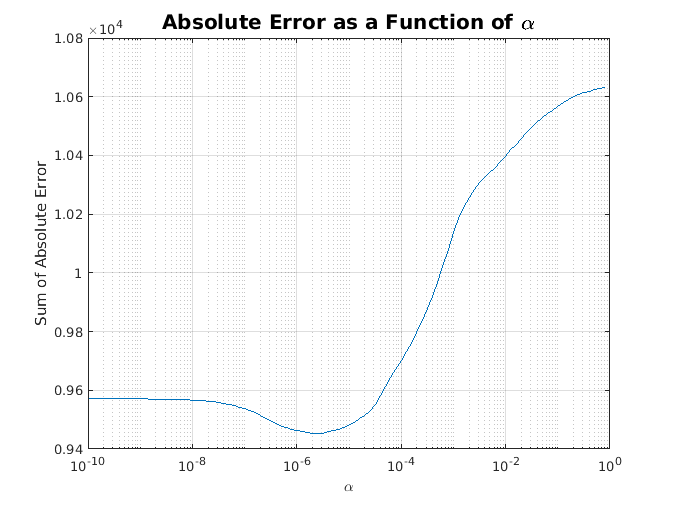
\includegraphics[width=\textwidth]{error-vs-alpha-order-3.png}
	\caption{$\bm{e}$ = $f(\alpha)$}
	\label{fig:error-vs-alpha-order-3}
    \end{subfigure}
    ~ 
	\begin{subfigure}[b]{0.3\textwidth}
        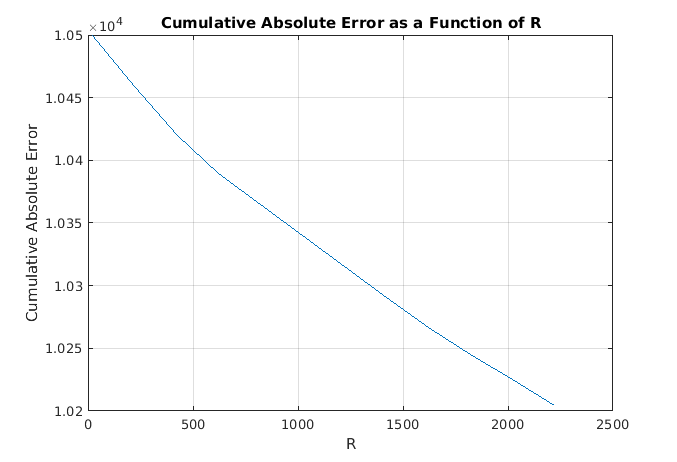
\includegraphics[width=\textwidth]{error-vs-r.png}
	\caption{$\bm{e}$ = $f(R)$}
	\label{fig:error-vs-r}
    \end{subfigure}
	\caption{Tuning $\alpha$ and $R$}
	\label{fig:tuning-alpha-r}
\end{figure}

Now we can also observe from Figure \ref{fig:error-vs-alpha-order-3} that error changes as the choice of $\alpha$ changes. The $\alpha$ choice is rather arbritrary and needs tuning. As I mentioned earlier, I chose $\alpha$ = $10^{-3}$ for all orders, since it seemed reasonable at most orders. Similarly, I plotted the error by varying $R$ = $(20:200:2000)$. Figure \ref{fig:error-vs-r} shows the effect of tuning $R$. I have chosen the noise variance of an autoregression model to be the effective $R$ after this observation.\\

\begin{figure}[!h]
    \centering
	\begin{subfigure}[b]{0.3\textwidth}
        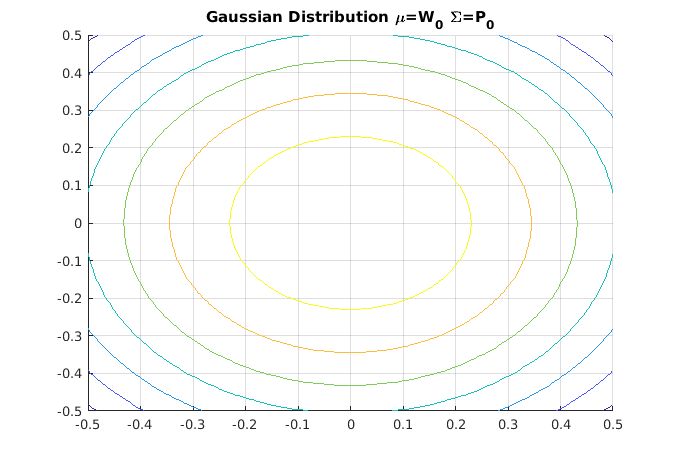
\includegraphics[width=\textwidth]{kalman-parameter-contour-initial.png}
	\caption{Initial Parameter Contour}
	\label{fig:kalman-parameter-contour-initial}
    \end{subfigure}
    ~ 
	\begin{subfigure}[b]{0.3\textwidth}
        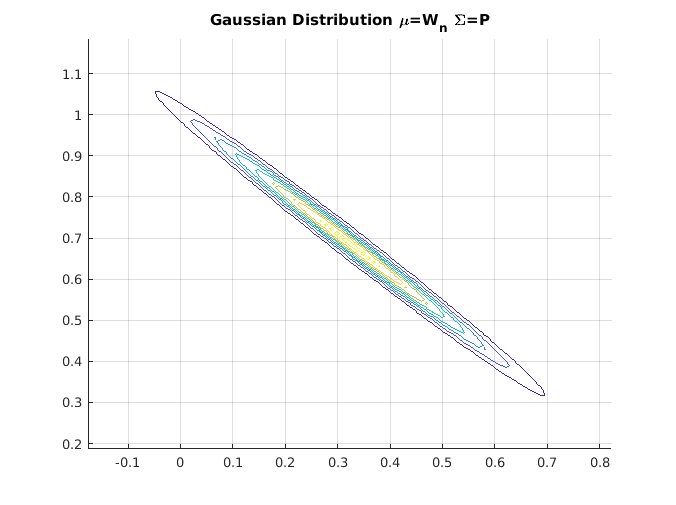
\includegraphics[width=\textwidth]{kalman-parameter-contour.png}
	\caption{Final Parameter Contour}
	\label{fig:kalman-parameter-contour}
    \end{subfigure}
	\caption{Parameter Contour Updates}
	\label{fig:kalman-parameter}
\end{figure}

Finally, from Figure \ref{fig:kalman-parameter}, we can clearly see the updates on the parameters. This diagram shows the spread of the parameters at the start and at the end of the kalman filter. We can clearly see how the spread has been shrinked into the final shape from the initial uniform shape. This is exactly as expected.\\

Overall, the benefit of building a kalman filter to deal with financial time series is that we can isolate the noise and tune the process of doing so. At the same time we receive a distribution of our solution, which tells us the confidence in the parameters. This way we may be able to make better judgements. However, we are yet to explain the residual noise.

\section{Predicting the Residual in Kalman Filter}

\begin{figure}[!h]
    \centering
    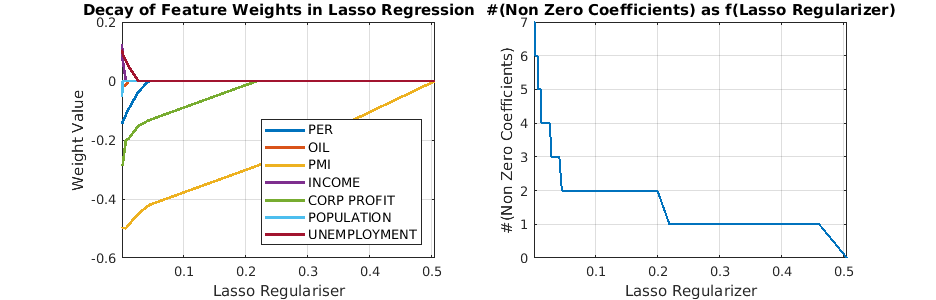
\includegraphics[width=0.8\textwidth]{decay-lasso.png}
	\caption{Decaying Features in Lasso Regulariser}
	\label{fig:decay-lasso}
\end{figure}

\begin{figure}[!h]
    \centering
	\begin{subfigure}[b]{0.3\textwidth}
        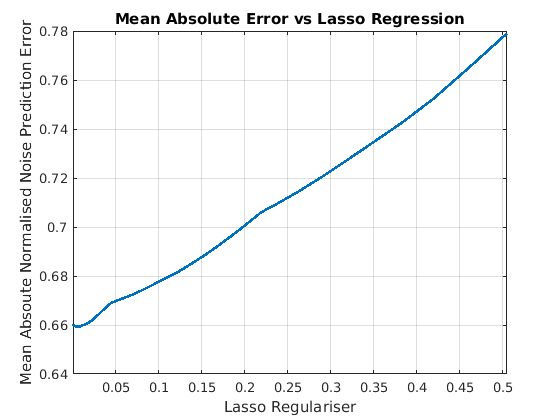
\includegraphics[width=\textwidth]{error-vs-lambda.png}
	\caption{Lambda vs Noise Prediction Error}
	\label{fig:error-vs-lambda}
    \end{subfigure}
    ~ 
	\begin{subfigure}[b]{0.3\textwidth}
        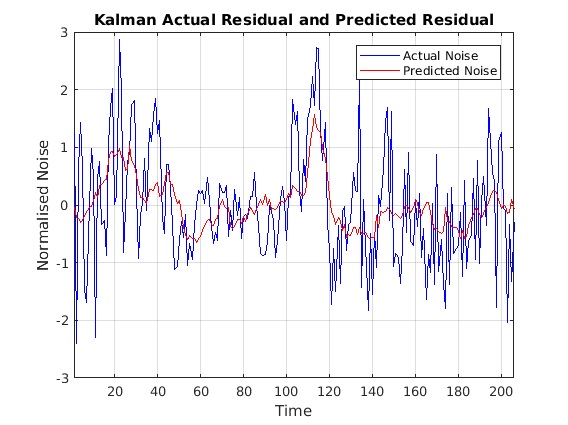
\includegraphics[width=\textwidth]{noise-prediction.png}
	\caption{Kalman Noise Prediction by Lasso}
	\label{fig:noise-prediction}
    \end{subfigure}
 	~ 
	\begin{subfigure}[b]{0.3\textwidth}
        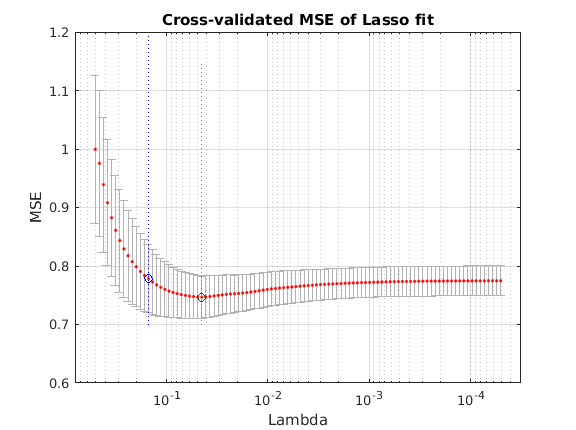
\includegraphics[width=\textwidth]{mse-lasso.png}
	\caption{Lasso Plot with Cross-Validated Fits}
	\label{fig:mse-lasso}
    \end{subfigure}
	\caption{Lasso Plots}
	\label{fig:lasso-figs}
\end{figure}

\begin{figure}[!h]
    \centering
    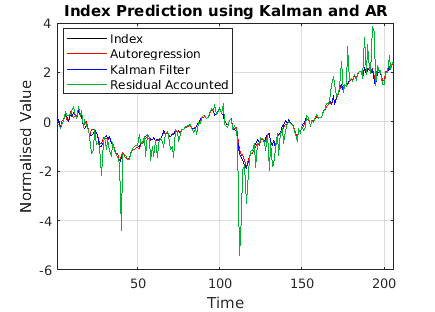
\includegraphics[width=0.5\textwidth]{laglasso.png}
	\caption{Two Months Lagged Residual Prediction Added to 2nd Order Kalman Filter Prediction}
	\label{fig:laglasso}
\end{figure}

\begin{thebibliography}{9}
\bibitem{mahler} 
N. Mahler, "Modeling the S \& P 500 index using the Kalman filter and the LagLasso," in \textit{Machine Learning for Signal Processing, 2009. MLSP 2009. IEEE International Workshop on, Sept 2009}, pp. 1–6.

\end{thebibliography}

\end{document}












































